	\documentclass[twoside]{article}
\usepackage{../../estilo-ejercicios}

%--------------------------------------------------------
\begin{document}

\title{Tarea}
\author{Javier Aguilar Martín}
\maketitle


\begin{ejercicio}{1}
Encontrar un algoritmo de complejidad lineal para resolver el problema del mínimo círculo generador de $n$ puntos. 
\end{ejercicio}
\begin{solucion}
Dados $n$ puntos $(a_i,b_i)\in\R^2$, $i=1,\dots, n$, buscamos el círculo más pequeño que los encierre a todos. Esto es equivalente a buscar un punto $(x,y)\R^2$ que minimice $\max\{(x-a_i)^2+(y-b_i)^2: 1\leq i\leq n\}$.\\

\textbf{Versión restringida del problema}

Primero vamos a resolver una versión restringida del problema, concretamente un caso en el que el céntro del círculo está necesariamente en una determinada recta. Por simplicidad fijaremos el eje $X$ como recta. Al final del cálculo, esta solución nos dirá en qué lado de la recta estará el centro en el caso no  restringido. 

Consideremos entonces el problema de minimizar $g(x)=\max\{(x-a_i)+b_i^2:1\leq i\leq n\}$. Sean $i,j$ dos índices distintos y consideremos la ecuación $(x-a_i)^2+b_i^2=(x-a_j)+b_j^2$, que desarrollando nos da la ecuación lineal $-2a_ix+a_i^2+b_i^2=-2a_jx+a_j^2+b_j^2$. Si $a_i=a_j$, entonces (suponiendo por ejemplo que $b_i^2\leq b_j^2$) podemos eliminar la función $(x-a_i)+b_i^2$ de la definición de $g$. Si $a_i\neq a_j$, entonces hay un valor crítico 
\[
x_{ij}=\frac{a_j^2-a_i^2+b_j^2-b_i^2}{2(a_j-a_i)}
\]
tal que (suponiendo que $a_j>a_i$) $(x-a_i)^2+b_i^2\geq (x-a_j)^2+b_j^2$ si y solo si $x\geq x_{ij}$. 

El algoritmo para el problema restringido funciona de la siguiente manera: Consideremos los pares $(1,2),(3,4),\dots$. Para cada par $(i,i+1)$ ($i$ impar) tal que $a_i=a_{i+1}$, eliminar una de las funciones como hemos explicado arriba. Calcular los valores críticos $x_{i,i+1}$. Encontrar la mediana $x_m$ de los valores $x_{i,i+1}$ con cualquier algoritmo de tiempo lineal (ver [AHU]). Sea $x^*$ el punto donde $g$ alcanza el mínimo. Clacular $g(x_m)$. Tenemos que discutir ahora la cuestión de determinar si $x_m<x^*$, $x_m=x^*$ o $x_m>x^*$. Sea $I=\{i:(x_m-a_i)^2+b_i^2=g(x_m)\}$. Si $x_m<a_i$ para todo $i\in I$ entonces $x_m<x^*$; si $x_m>a_i$ para todo $i\in I$ entonces $x_m>x^*$; en otro caso $x_m=x^*$. Sabiendo que $x^*<x_m$ o que $x^*>x_m$ podemos descartar una cuarta parte de las funciones de la siguiente forma. Supongamos por ejemplo que $x^*<x_m$. Tenemos al menos la mitad de nuestro valores críticos $x_{i,i+1}$ mayores que $x^*$. Si $x_{i,i+1}>x_m$ entonces, como $(x-a_i)^2+b_i^2\geq (x-a_{i+1})^2+b_{i+1}^2$ si y solo si $x\geq x_{i,i+1}$, podemos descartar la función $(x-a_i)^2+b_i^2$. Esto se debe a que $(x^*-a_i)+b_i^2\leq (x^*-a_{i+1})^2+b_{i+1}^2$. Así que para al menos la mitad de los pares podemos descartar una función de cada par. Esto implica que al menos una cuarta parte de las funciones son descartadas al final de este paso, de lo que se sigue la linealidad en el tiempo de ejecución.\\

Tratamos ahora la cuestión de reconocer en qué lado de la línea recta se encuentra el centro del problema sin restringir. Primero, obsérvese que la función $f(x,y)=\max\{(x-a_i)^2+(y-b_i)^2:i\leq i\leq n\}$ es convexa. Es esencial notar que $f$ es convexa, no solo en cada variable, sino como función de dos variables. Esto implica que la función $h(y)=\min_x f(x,y)$ es convexa. Minimizando $g(x)$ de hecho evaluamos $h(0)$. La coordenada $y$ del problema no restringido es precisamente donde $h(y)$ alcanza el mínimo. Denotamos este valor como $y^c$. Como $h(y)$ es convexa, podemos determinar el signo de $y^c$ simplemente mirando en un entorno de $y=0$. Por tanto, sea $(x^*,0)$ el centro del problema restringido que habíamos encontrado previamente. Sea $I=\{i:(x^*-a_i)^2+b_i^2=g(x^*)\}$. Obviamente, si $I=\{i\}$ entonces $x^*=a_i$ e $y^c$ tiene el signo de $b_i$. Si $I=\{i,j\}$ entonces $(x^*,0)$ se encuentra en la mediatriz del segmento $[(a_i,b_i),(a_j,b_j)]$. Obviamente, $y^c$ tiene el signo de la coordenada $y$ del punto medio de este segmento, es decir, de $\frac{1}{2}(b_i+b_j)$. En general, todos los puntos $(a_i,b_i)$ con $i\in I$ se encuentran dentro de un círculo centrado en $(x^*,0)$. Si $(x^*,0)$ está en la envolvente convexa de estos puntos entonces $y^c=0$. En otro caso, existen dos puntos $(a_i,b_i)$, $(a_j,b_j)$ ($i,j\in I$) tales que $f(x,y)$ decrece a medida que nos movemos desde $(x^*,0)$ en la dirección del punto medio del segmento $[(a_i,b_i),(a_j,b_j)]$ (es decir, a lo largo de la mediatriz de ese segment, ver Figura \ref{Fig4}). En este caso $y^c$ tiene el signo de $\frac{1}{2}(b_i+b_j)$. Debe tenerse en cuenta que la determinación de estos dos puntos o la determinación de que $(x^*,0)$ está en la envolvente convexa puede ser llevada a cabo en tiempo lineal (ver [NME]).


\begin{figure}[h!]
\centering
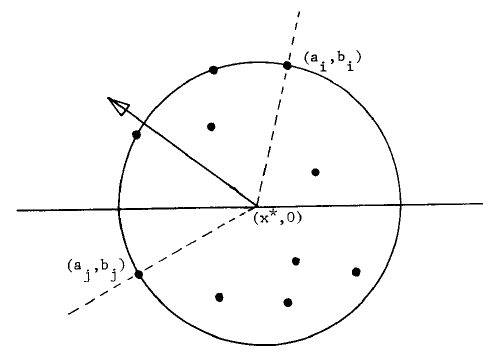
\includegraphics[scale=0.7]{Fig4}
\caption{}\label{Fig4}
\end{figure}
  \newpage
  En resumen, dada cualquier recta en el plano, podemos en $O(n)$ determinar en qué lado de la recta está el centro del mínimo círculo generador. Además, si este centro resulta estar en la recta descubriríamos su localización exacta durante el proceso.\\
  
  \textbf{Algoritmo lineal para el mínimo círculo generador} 
  Utilizaremos ahora el resultado anterior para encontrar el centro del problema no restringido. Empezamos creando las mediatrices de los segmentos $[(a_{2i-1},b_{2i-1}),(a_{2i},b_{2i})]$, $i=1,\dots, \lfloor n/2\rfloor$. Las denotamos por $L_i$. Consideremos los ángulos $\alpha$ ($-\pi/2\leq\alpha\leq\pi/2$) que forman las mediatrices con la dirección positiva del eje $X$. Sean $\alpha_m$ la mediana de estos ángulos. Consideremos la transformación lineal que lleva el eje $x$ a la recta $y=\alpha_mx$ y deja fijo el eje $Y$. Aplicando esta transformación podemos tener al menos la mitad de nuestras mediatrices con ángulos no negativos y al menos la mitad de ellas con ángulos no positivos. Es obvio que esto se puede conseguir en tiempo lineal.
  
  El siguiente paso es formar pares disjuntos de rectas $(L_i,L_j)$ de modo que cada par tenga una recta con ángulo no negativo y otra con ángulo no positivo. Por tanto habrá $\lfloor n/4\rfloor$ tales rectas. Para cada par $(L_i,L_j)$ definimos el valor $y_{ij}$ como sigue. Si $L_i$ y $L_j$ son paralelas al eje $X$ sea entonces $y_{ij}$ la media de sus coordenadas $y$ (que son constantes). En otro caso debe cortarse en un punto que denotamos $(x_{ij},y_{ij})$. Ahora, sea $y_m$ la mediana de los $\lfloor n/4\rfloor$ valores $y_{ij}$. El valor $y_m$ puede ser encontrado en tiempo lineal. Ahora buscamos en qué lado de la recta $y=y_m$ se debe encontrar el centro. Este proceso tiene complejidad $O(n)$ como hemos comentado en el apartado anterior. Si el centro se encuentra en la recta $y=y_m$ ya hemos terminado. Por lo tanto, supongamos que no se encuentra sobre la recta sino que, por ejemplo, se encuentra debajo de ella. Consideremos un par $(L_i,L_j)$ de rectas paralelas (si existen) tales que $y_{ij}\geq y_m$. Al menos una de estas rectas está por encima de $y=y_m$, digamos $L_i$ (que es perpendicular a la mediatriz del segmento $[(a_{2i-1},b_{2i-1}),(a_{2i},b_{2i})]$). Podemos ahora eliminar uno de estos dos puntos, concretamente el que está debajo de $L_i$, ya que el otro punto está más lejos del centro. Sin embargo, en general $L_i$ y $L_j$ no son paralelas. 
  
  Consideremos ahora el conjunto de todos los pares $(L_i,L_j)$ de rectas no paralelas para los cuales $y_{ij}\geq y_m$. Calculamos la mediana $x_m$ de las  correspondientes $x_{ij}$. Igual que en el caso de la coordenada $y$, comprobamos en qué lado de la recta $x=x_m$ está el centro del círculo mínimo generador. Supongamos por ejemplo que se encuentra a la izquierda de esta recta. Consideremos los pares $(i,j)$ tales que $x_{ij}\geq x_m$ e $y_{ij}\geq y_m$. Una de estas rectas, digamos $L_i$, forma un ángulo no positivo con la dirección positiva del eje $X$. Se sigue (ver Figura \ref{Fig5}) que uno de los puntos que definen $L_i$, en concreto, el que está en el ``suroeste'', puede ser eliminado ya que el otro punto estará al menos tan lejos como este del centro.
  
  \begin{figure}[h!]
  \centering
  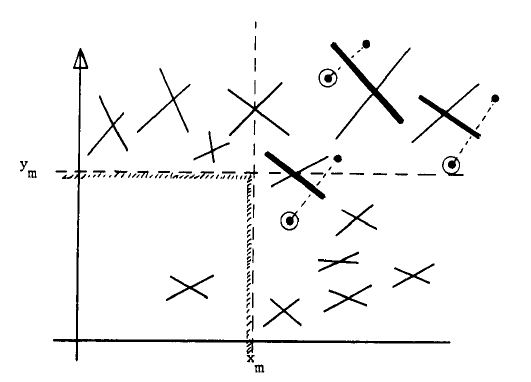
\includegraphics[scale=0.7]{Fig5}
  \caption{}\label{Fig5}
  \end{figure}
  
  Se sigue que durante este proceso nos deshacemos de un punto de cada par para al menos una cuarta parte de los pares de rectas. En otras palabras, al menos $\lfloor n/16\rfloor$ puntos serán eliminados con un tiempo de ejecución de $O(n)$. Se sigue por tanto que el proceso completo se realiza en $O(n)$. \\
 
 \textbf{Referencias}
 
[NME] N. Megiddo, ``Linear-time algorithms for linear programming in $\R^3$ and related problems'', 23rd Annual Symposium on Foundations of Computer Science (sfcs 1982), Chicago, IL, USA, 1982, pp. 329-338.
doi: 10.1109/SFCS.1982.24

[AHU] A. V. Aho, J. E. Hopcroft, J. D. Ullman. ``The Design and Analysis of Computer Algorithms'', Addison-Wesley, Reading, MA, 1974. 
\end{solucion}



\end{document}
